Notre approche vise à maximiser l'utilisation des dépendances et complémentarités entre différents types de données (vidéo, texte,
audio). Pour effectuer des prédictions en utilisant ces diverses modalités, nous avons opté pour l'utilisation de chaque réseau de
neurones présentés précédemment afin d'extraire des représentations compressées (ou features) des différents types de données. 

Les modèles individuels sont initialement pré-entraînés, puis fusionnés en une seule architecture multimodale qui subit ensuite un
nouvel entraînement. Le pré-entraînement des modèles individuels présente l'avantage de réduire le temps de convergence de
l'entraînement de cette architecture multimodale comprenant un nombre important de paramètres.

Au cours de ce processus, pour des raisons de contraintes de ressources, on gèle les poids des modèles unimodaux.

\subsection{Le LATE FUSION}
Ce premier modèle multimodal fait passer chaque donnée dans son modèle pré-entraîné associé et fait une moyenne des sorties. Le but
est alors de faire une moyenne des probabilités selon chaque canal. Nous appellerons ce modèle \textit{LATE FUSION}, du fait que la 
fusion se fasse à la fin. Comme ce modèle utilise seulement les modèles unimodaux pré-entrainés, il n'y a pas besoin de faire 
d'apprentissage sur ce modèle.
La Figure~\ref{fig: LATE FUSION} résume l'architecture de ce modèle.

\begin{figure}[H]
    \centering
    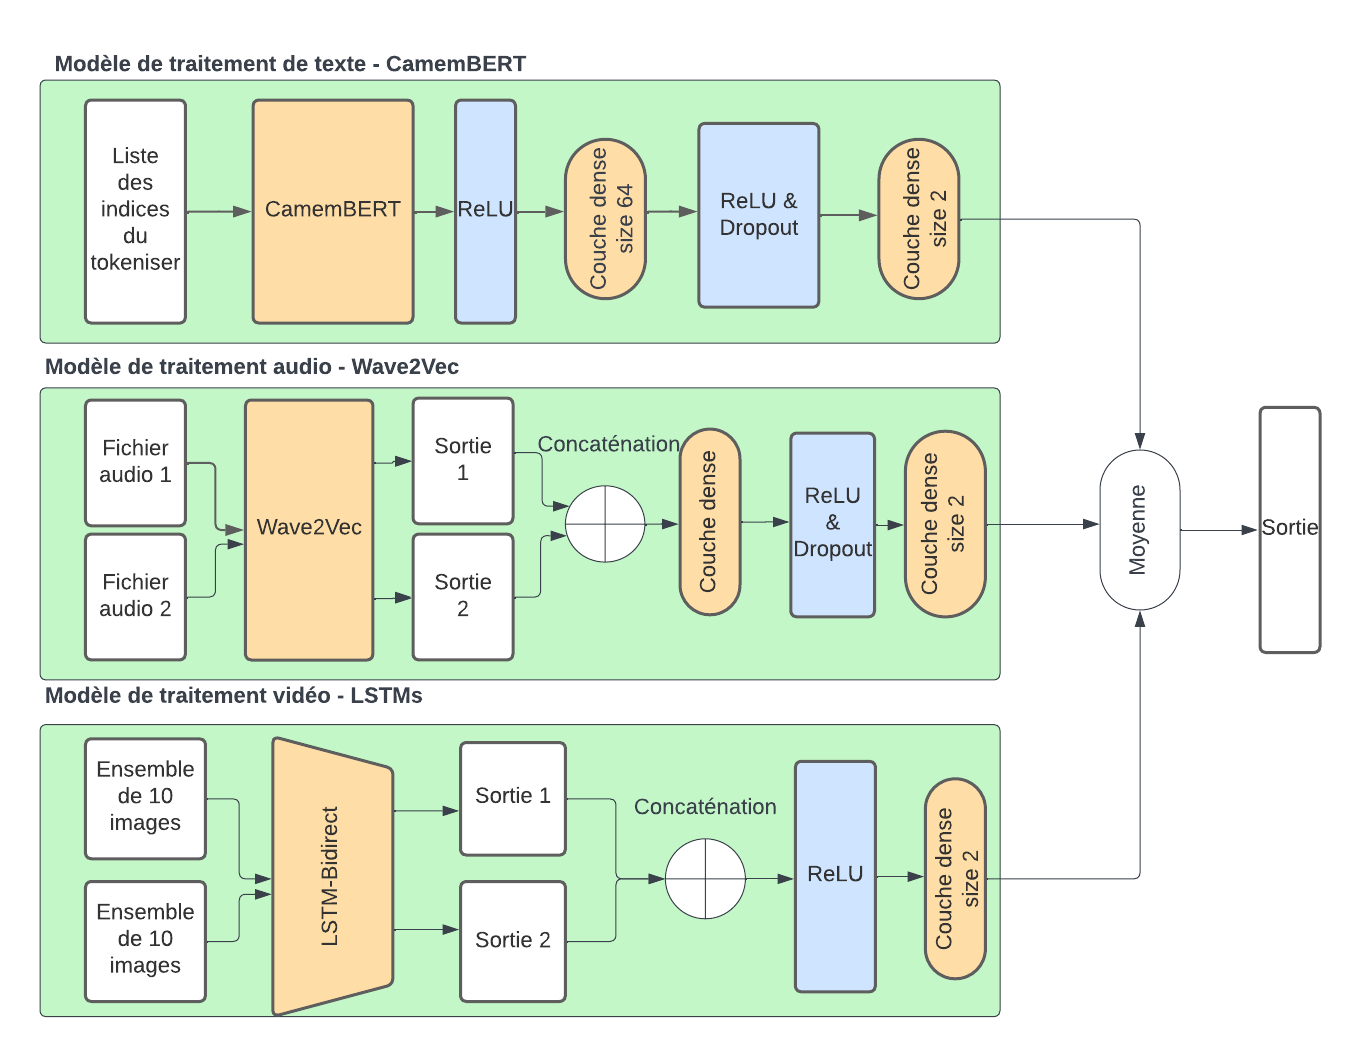
\includegraphics[width=0.6\textwidth]{image_model/late_fusion.png}
    \caption{Architecture du modèle \textit{LATE FUSION}}
    \label{fig: LATE FUSION}
\end{figure}

\subsection{L'EARLY FUSION}
Ce deuxième modèle plus évolué consiste à faire passer chaque donnée dans son modèle pré-entraîné associé et de récupérer
l'information avant qu'elle ne passe dans la dernière couche dense (celle de taille deux). On concatène alors toute l'information 
et on la fait passer dans une grande couche dense de taille 2.
La Figure~\ref{fig: EARLY FUSION} résume l'architecture de ce modèle, qu'on appellera \textit{EARLY FUSION}, du fait que la fusion
se passe avant les couches de neurones.

\begin{figure}[H]
    \centering
    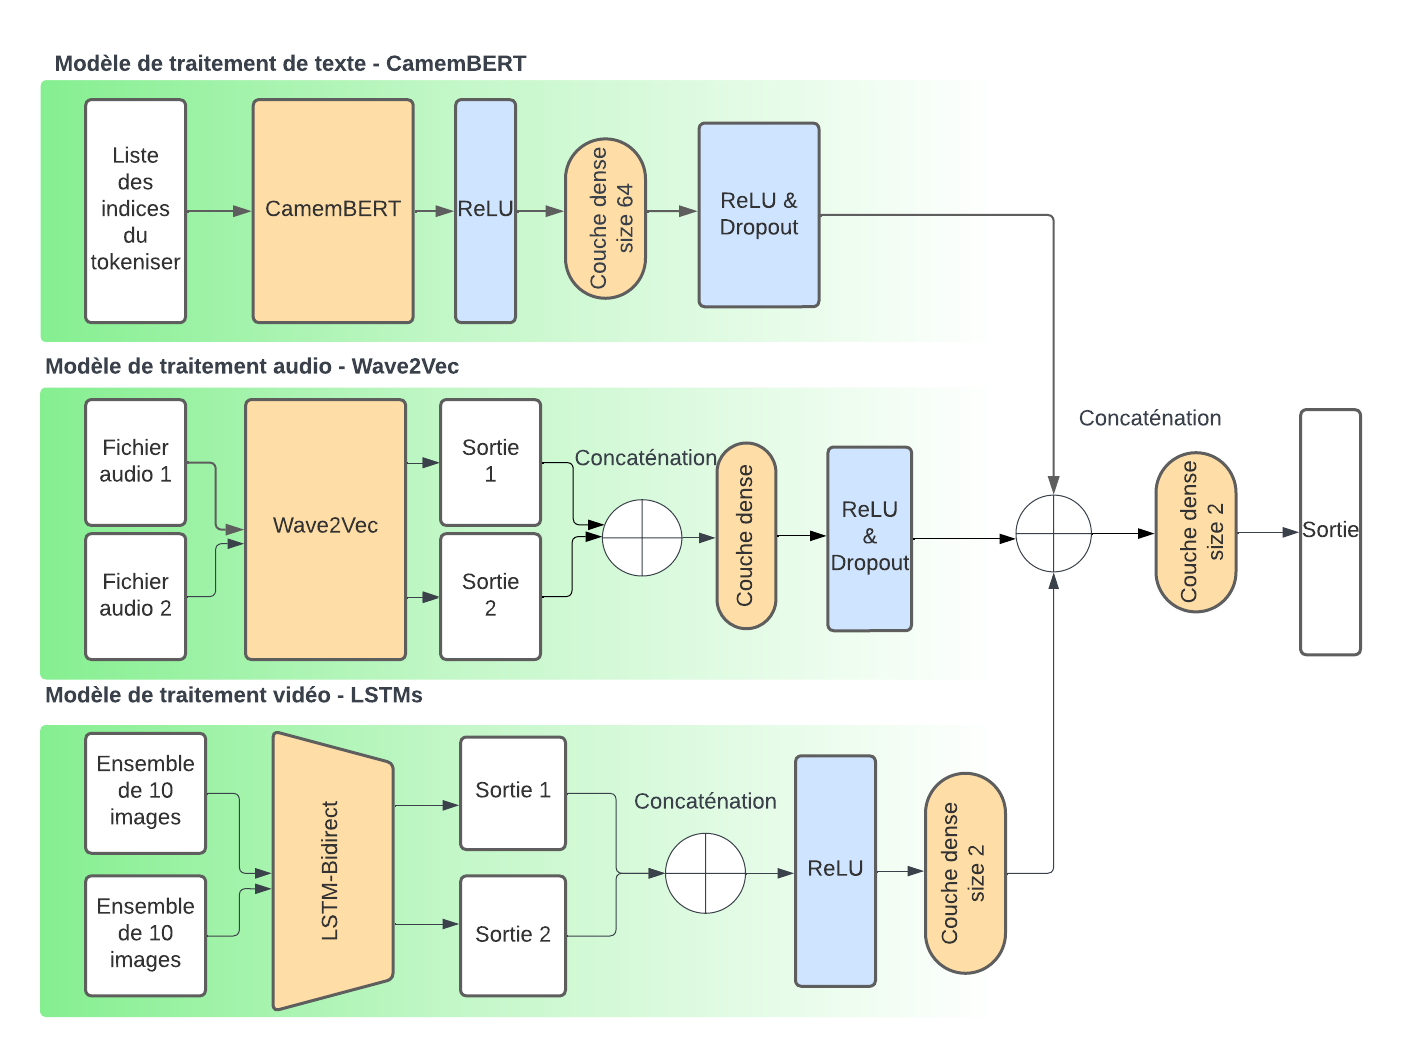
\includegraphics[width=0.6\textwidth]{image_model/early_fusion.png}
    \caption{Architecture du modèle \textit{EARLY FUSION}.}
    \label{fig: EARLY FUSION}
\end{figure}